\chapter{Analiza matematyczna}

Materiały teoretyczne z analizy matematycznej zostały opracowane na podstawie \href{https://www.mimuw.edu.pl/~pawelst/dydaktyka/}{skryptu Pawła Strzeleckiego}, oryginalnych prac Eulera, Weierstrassa, Darboux, Rolle'a i Lagrange'a oraz \href{https://docs.google.com/document/d/1zH2fxnEpsVWZCMUf7qZtla7rl0BFxe-I6gzpkSep8nk}{tego dokumentu}.

\section*{Podstawa programowa}
\begin{enumerate}
    \item \textbf{Granica} ciągu.
    \item \textbf{Szeregi} liczbowe, zbieżność bezwzględna i warunkowa.
    \item \textbf{Ciągłość} i \textbf{jednostajna ciągłość} funkcji i najważniejsze własności funkcji ciągłych.
    \item \textbf{Pochodna funkcji jednej zmiennej}, interpretacja geometryczna i mechaniczna.
    \item \textbf{Twierdzenie Lagrange’a o wartości średniej}, jego interpretacja geometryczna i niektóre konsekwencje (monotoniczność, wklęsłość, wypukłość, szacowanie przyrostów).
    \item \textbf{Wzór Taylora} dla funkcji jednej zmiennej, zastosowania do obliczeń przybliżonych, rozwijanie funkcji w \textbf{szeregi potęgowe}.
    \item Pojęcie \textbf{zbieżności ciągów} liczbowych i funkcyjnych, twierdzenia o przejściu do granicy pod znakiem pochodnej i całki.
    \item \textbf{Ekstrema funkcji} jednej i kilku zmiennych rzeczywistych: warunki konieczne i dostateczne.
    \item \textbf{Funkcja pierwotna, całka oznaczona}. Zastosowania geometryczne całki.
    \item \textbf{Elementy teorii miary}.
\end{enumerate}

\section{Granica ciągu}
\subsection{Podstawowe informacje}
Ciąg $(a_n)\subset \RR$ jest \textbf{zbieżny do granicy} $a \in \RR \Longleftrightarrow$
$$
\purple{\forall \epsilon > 0 \quad \exists N_0 \in \NN \quad \forall n > N_0: \quad |a_n - a| < \epsilon}
$$
zapisujemy 
$$
\lim_{n\to\infty}a_n = a, \qquad a_n \to a \ (\mbox{dla } n\to\infty)
$$
dla liczb zespolonych analogicznie.

\begin{figure}[h]
    \centering
    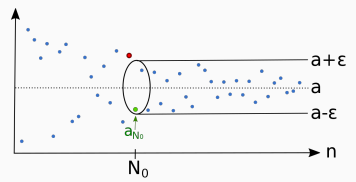
\includegraphics[scale=0.5]{rozdziały/images/Analiza/granica_ciagu_shooter.png}
\end{figure}

\textbf{Wnioski} 
\begin{itemize}
    \item Każdy ciąg \textbf{zbieżny jest ograniczony} (poza ustalonym paskiem jest tylko skończenie wiele $a_n$). 
    \item Ciąg zbieżny ma \textbf{jedną} granicę.
\end{itemize}
\begin{example}
    $$
    \lim_{n\to\infty}\frac{1}{n}=0, \qquad \lim_{n\to\infty}\sqrt[n]{n}=1, \qquad \mbox{dla } q\in(-1,1) \ \lim_{n\to\infty}q^n = 0, \ \lim_{n\to\infty}n^kq^n=0
    $$
\end{example}
\textbf{Własności arytmetyczne granicy}:
Jeśli $a_n \to a$ oraz $b_n \to b$, to
\begin{itemize}
    \item $a_n \pm b_n \to a \pm b$
    \item $a_n\cdot b_n \to a \cdot b$
    \item $\frac{a_n}{b_n}\to \frac{a}{b}$ o ile $b_n, b \neq 0$
\end{itemize}
\subsection{Ważne twierdzenia}
\textbf{Twierdzenie o trzech ciągach/dwóch policjantach}:
Jeśli $b_n \le a_n \le c_n$ dla $n\ge N_1$ oraz $b_n, c_n \to a$, to także $a_n \to a$
\begin{example}
\begin{itemize}
    \item $\sqrt[n]{69}\to 1$, bo dla $n>69$ zachodzi $1 < \sqrt[n]{69} < \sqrt[n]{n}$ oraz $1\to 1, \sqrt[n]{n}\to 1$
    \item $\sqrt[n]{3^n + 5^n + 8^n}\to 8$, bo $8=\sqrt[n]{8^n} \le \sqrt[n]{3^n + 5^n + 8^n} \le \sqrt[n]{3 * 8^n} = \sqrt[n]{3}* 8\to 8 $
\end{itemize}
\end{example}
\begin{exam}
    Ciąg, którego $n$-ty wyraz zadany jest wzorem $\sqrt{n^2+(-1)^n}-n$
    \answers{jest monotoniczny}{jest rozbieżny}{jest nieograniczony}
    Zastosujemy twierdzenie o trzech ciągach. Widzimy, że $\sqrt{n^2 - 1} - n \le \sqrt{n^2 - (-1)^n} - n \le \sqrt{n^2 + 1} - n$. Pozostaje tylko pokazać granice policjantów. Mamy $\sqrt{n^2 - 1} - n = \frac{(\sqrt{n^2 - 1} - n)(\sqrt{n^2 - 1} + n)}{\sqrt{n^2-1}+n}=\frac{-1}{\sqrt{n^2-1}+n} \to 0$. Dla $(+1)$ tak samo. W takim razie \textbf{B} i \textbf{C} to \texttt{NIE}. Czy ciąg jest monotoniczny? $a_1 = -1 < 0, \ a_2=\sqrt{4 + 1} - 2 > 0, \ a_3=\sqrt{9-1}-3=\sqrt{8}-3 < 0$. Nie jest. Zatem \textbf{A} to też \texttt{NIE}.
\end{exam}
\textbf{Twierdzenie Bolzano-Weierstrassa}:
Każdy ciąg ograniczony ma podciąg zbieżny.

\textbf{Twierdzenie}:
Każdy ciąg monotoniczny i ograniczony ma granicę (skończoną).
\begin{example}
\begin{itemize}
    \item $a_1=2, \quad a_{n+1}=\sqrt{6 + a_n} \ \Longrightarrow a_n \to 3$
    \item $b_1=2, \quad b_{n+1}=12 + \frac{b_n}{7} \ \Longrightarrow b_n \to 14$
    \item $c_1=2, \quad c_{n+1}=\frac{c_n^2 + 2}{2c_n} \ \Longrightarrow c_n \to \sqrt{2}$
\end{itemize}
Jak to wykazać? Analiza dla $c_n$
\begin{itemize}
    \item Widać, że wszystkie $c_n>0$
    \item Monotoniczność: $c_{n+1} < c_n$, po indukcji: $c_{n+1} \stackrel {?}{<} c_n$ wtedy $c_n-c_{n+1}>0$, czyli $c_n-\frac{c_n^2+2}{2c_n}=\frac{2c_n^2-c_n^2-2}{2c_n}=\frac{c_n^2-2}{2c_n}>0$, co zachodzi jedynie gdy $c_n > \sqrt{2}$
    \item Czy faktycznie $c_n>\sqrt{2}$? Indukcja: $c_1=2>\sqrt{2}$ -- baza ok. Zał. $c_n>\sqrt{2}$, $c_{n+1}-\sqrt{2}=\frac{c_n^2+2}{2c_n}-\sqrt{2}=\frac{c_n^2-2c_n\sqrt{2} + 2}{2c_n} = \frac{(c_n-\sqrt{2})^2}{2c_n}>0$
\end{itemize}
Wszystkie wyrazy ciągu są $>\sqrt{2}$ i jest on malejący, zatem $c_n\to \sqrt{2}$.
\end{example}

\subsection{Ciągi Cauchy'ego}
$(a_n) \subset \RR$ spełnia \textbf{warunek Cauchy'ego} (jest ciągiem Cauchy'ego) $\Longleftrightarrow$
$$
\purple{\forall \epsilon > 0 \quad \exists N_0\in \NN \quad \forall m,n > N_0: \quad |a_n-a_m| < \epsilon}
$$
Intuicyjnie: dalekie wyrazy różnią się dowolnie mało.

\textbf{Stwierdzenie:} każdy ciąg Cauchy'ego jest ograniczony.

\textbf{Twierdzenie:} Ciąg w $\RR$ (w $\CC$) jest zbieżny $\Longleftrightarrow$ jest ciągiem Cauchy'ego.

\subsection{Exp i ln}
\textbf{Definicja:} $$e^x=\exp(x) := \lim_{n\to\infty}\left(1 + \frac{x}{n}\right)^n$$
\textbf{Twierdzenie:} $\exp$ jest różnowartościową surjekcją na $(0, \infty)$.

\textbf{Definicja:} 
$$
ln = (\exp)^{-1}: \ (0, \infty) \to \RR
$$

\begin{problems}
    \prob Jeśli ciąg liczb rzeczywistych dodatnich $a_n$ jest monotoniczny i ograniczony, to
    \answers{ciąg $\sin (a_n)$ jest monotoniczny}{ciąg $\cos (a_n)$ jest zbieżny}{ciąg $\log (a_n)$ jest ograniczony} % nie tak nie

    \prob Ciąg, którego $n$-ty wyraz zadany jest wzorem $\cfrac{2010^n - n^{2010}}{2^{n^2}-2010^n}$,
    \answers
    {jest zbieżny}
    {ma granicę równą $-1$}
    {ma granicę równą 0}

    \prob Niech $\{a_n\}_{n \geq 0}$ będzie ograniczonym ciągiem dodatnich liczb rzeczywistych. Wtedy
    \answers{jeśli $\{\sin(a_n)\}_{n \geq 0}$ jest zbieżny, to $a_n$ jest monotoniczny}{$\{\exp(-a_n)\}_{n \geq 0}$ posiada podciąg zbieżny do granicy dodatniej}{jeśli $\{\exp(-a_n)\}_{n \geq 0}$ jest zbieżny, to $\{\arctan(a_n)\}_{n \geq 0}$ ma granicę dodatnią}

    \prob Ciąg określony dla $n \geq 1$ wzorem $(1+\frac{1}{4^n})^{2^n}$ jest
    \answers{zbieżny do 1}{rosnący, począwszy od pewnego miejsca}{ograniczony}

    \prob Ciąg $a_n = \left(0.999 + \frac{1}{4n}\right)^{4n}$
    \answers{jest zbieżny do liczby większej od 0}{jest zbieżny do liczby niewymiernej}{jest ograniczony z góry}
\end{problems}

\section{Szeregi o wyrazach dodatnich}
\subsection{Definicje}
Szereg $$\purple{\sum_{n=1}^{\infty}a_n}$$ to \textbf{para ciągów}, $(a_n)\subset \RR$ (lub $\CC$) oraz $$\purple{s_n = a_1 + \dots + a_n = \sum_{k=1}^na_k}, \ n \in \NN,$$ gdzie $\purple{s_n}$ to \textbf{sumy częściowe szeregu} $\purple{a_n}$ to \textbf{wyrazy szeregu}. 

Szereg $\sum_{n=1}^na_n$ jest \textbf{zbieżny} $\Longleftrightarrow$ sumy częściowe $s_n$ mają skończoną granicę s. Zapis: $s=\lim_{n\to\infty}s_n=\sum_{n=1}^{\infty}a_n$
\subsection{Warunki zbieżności}
\begin{itemize}
    \item warunek konieczny: jeśli szereg $\sum_{n=1}^{\infty}a_n$ jest zbieżny, to $\lim_{n\to\infty}a_n=0$
    \item warunek dostateczny (warunek Cauchy'ego dla szeregów): $\sum_{n=1}^{\infty}a_n$ jest zbieżny $\Longleftrightarrow$ zachodzi \textbf{warunek Cauchy'ego dla szeregów}
\end{itemize}
\textbf{Warunek Cauchy'ego:} dla kazdego $\epsilon > 0$ istnieje $n_{\epsilon}\in \NN$ takie, że dla $m > k > n_{\epsilon}$ jest 
$$
|a_{k+1}+a_{k+2}+\dots+a_m| < \epsilon
$$
\textbf{Równoważne warunki:}
\begin{itemize}
    \item szereg $\sum_{n=1}^{\infty}a_n$ jest zbieżny
    \item Ciąg $(s_n)$ jest ograniczony z góry (\textbf{mówimy o szeregach dodatnich})
    \item $\sup{s_n : n\in\NN}\in \RR$
\end{itemize}
\begin{example}
    Szereg harmoniczny jest rozbieżny, bo $\frac{1}{n+1} + \frac{1}{n+2}+\dots+\frac{1}{2n}> n \cdot \frac{1}{2n} =\frac{1}{2}$. Każdą paczkę $n$ składników możemy ograniczyć z dołu przez $\frac{1}{2}$. Dokładając kolejne paczki zwiększamy sumy częściowe, które zatem nie są ograniczone z góry.
\end{example}
\subsection{Kryteria zbieżności szeregów o wyrazach dodatnich}
\textbf{Kryterium zagęszczeniowe}

Jeśli $a_1 > a_2 > \dots > 0$, to szeregi
$$
\sum_{n=1}^{\infty}a_n \qquad \mbox{i} \qquad \sum_{n=1}^{\infty}2^na_{2^n}
$$
są jednocześnie \textbf{oba zbieżne, albo oba rozbieżne}.
\begin{example}
    Dla $a_n=\frac{1}{n}$ jest $2^na_{2^n}=2^n\cdot\frac{1}{2^n}=1$. Szereg $\sum 1$ jest rozbieżny, więc $\sum\frac{1}{n}$ także.
\end{example}
\textbf{Kryterium porównawcze}
Niech $a_n, b_n>0$ oraz $a_n\le c \cdot b_n$ dla $n\ge n_0$. Wtedy
$$
\sum_{n=1}^{\infty}b_n \mbox{ zbieżny } \Longrightarrow \sum_{n=1}^{\infty}a_n \mbox{ zbieżny }, \qquad 
\sum_{n=1}^{\infty}a_n \mbox{ rozbieżny } \Longrightarrow \sum_{n=1}^{\infty}b_n \mbox{ rozbieżny }
$$
\textbf{Kryterium porównawcze asymptotyczne}
Jeśłi $a_n, b_n>0$ dla $n\ge n_0$ oraz $\lim_{n\to\infty}\frac{a_n}{b_n}\in(0, +\infty),$ to $\sum a_n$ i $\sum b_n$ są oba zbieżne, \textbf{albo} oba rozbieżne.
\begin{example}
    $\sum\frac{1}{n^2}=1 + \frac{1}{2^2} + \frac{1}{3^2}+\dots+\frac{1}{n^2} < 1 + \frac{1}{1\cdot 2} + \frac{1}{2\cdot 3} + \dots + \frac{1}{n(n-1)}=1+(1-\frac{1}{2})+(\frac{1}{2}-\frac{1}{3})+\dots+(\frac{1}{n-1}-\frac{1}{n}) = 2-\frac{1}{n} < 2,$ czyli sumy częściowe są ograniczone, sztuczka z "teleskopowaniem".

    W ogólności $\sum\frac{1}{n^2}$ zbieżny dla $s>1$.
\end{example}
\begin{problems}
    \prob $\{S_n\}_{n\geq1}$ jest ciągiem sum częściowych szeregu rozbieżnego. Wynika z tego, że ciąg $\{S_{n+1} - S_n\}_{n\geq1}$ jest
    \answers
    {rozbieżny}
    {nieograniczony}
    {niezbieżny do 0}
\end{problems}

\section{Szeregi o wyrazach dowolnych}
\subsection{Rodzaje zbieżności}
\begin{itemize}
    \item szereg $\sum_{n=1}^{\infty}a_n$ jest \purple{bezwzględnie} zbieżny $\Longleftrightarrow \purple{\sum_{n=1}^{\infty}|a_n|<\infty}$
\item Szereg $\sum_{n=1}^{\infty}a_n$ jest \purple{warunkowo} zbieżny $\Longleftrightarrow $ jest zbieżny, ale \purple{nie bezwzględnie}
\end{itemize}
Naturalnie szereg zbieżny bezwzględnie jest zbieżny.
\subsection{Kryterium Leibniza}
\textbf{Twierdzenie:} jeśli $a_1 \ge a_2 \ge \dots \ge 0$ oraz $a_n \to 0$, to szereg $\sum_{n=1}^{\infty}(-1)^{n+1}a_n$ jest zbieżny.

\begin{example}
    Szereg anharmoniczny $\sum_{n=1}^{\infty}\frac{(-1)^{n+1}}{n}$ jest zbieżny (ale nie bezwzględnie). Zbieżność wynika wprost z kryterium Leibniza, a wiemy, że nie jest bezwzględnie zbieżny z działu o szeregach o wyrazach dodatnich.
\end{example}
\subsection{Kryterium Dirichleta}
\textbf{Twierdzenie Abela:}
$$(a_n), (b_n) \subset \CC, M > 0.$$
Niech $|A_n| = |a_1 + \dots + a_n| \le M$ dla $n\in \NN$, 
$$
\sum_{n=1}^{\infty}|b_n-b_{n+1}| < +\infty \ \mbox{  oraz  } \ b_n \to 0 \mbox{ dla } n \to \infty
$$
Wtedy $\sum a_n b_n$ jest zbieżny.
\textbf{Wniosek (kryterium Dirichleta)} jeśli $b_1 \ge b_2 \ge \dots \ge 0, b_n \to 0$ oraz $\sum a_n$ ma sumy częściowe wspólnie ograniczone (jak w tw. Abela), to $\sum a_n b_n$ jest zbieżny.
\begin{example}
    $z\in \CC, \ |z| = 1, \ z \neq 1$, to $\sum\frac{z^n}{n}$ jest zbieżny.  Bierzemy $a_n=z^n$ oraz $b_n=\frac{1}{n}$. Możemy oszacować $|1 + z + z^2 + \dots + z^n| = \frac{1-z^n}{1-z} \le \frac{2}{1-z}$ ograniczone, $b_n$ oczywiście zbiega do $0$.
\end{example}

\begin{problems}
    \prob Rozważmy szeregi:
    $$
    (A)\ \sum_{n=1}^{\infty}\frac{7^n+n^9+\ln(19^{n^2}+8)}{8^n-11^{\ln(1+n)}+2}\quad\text{oraz}\quad (B)\ \sum_{n=1}^{\infty}\frac{8^n-11^{\ln(1+n)}+2}{7^n+n^9+\ln(19^{n^2}+8)}
    $$
    \answers{ciąg sum częściowych każdego z tych szeregów jest ograniczony}{szereg $(A)$ jest zbieżny}{szereg $(B)$ jest zbieżny}
\end{problems}

\section{Ciągłość funkcji}

Powiemy, że $a$ jest \textbf{punktem skupienia} zbioru $A \subset \RR$ wtedy i tylko wtedy, gdy istnieje ciąg $(a_n) \subset A - \{a\}$, taki że $a_n \to a$.

\begin{example}
    \begin{itemize}
        \item Zbiór $\ZZ$ nie ma punktów skupienia.
        \item 0 jest jedynym punktem skupienia zbioru $A = \{\frac{1}{n} \ : \ n \in \NN\}$.
        \item Każde $a \in [p, q]$ jest punktem skupienia zbioru $(p, q)$.
        \item Każde $a \in \QQ$ jest punktem skupienia $\RR - \QQ$, bo np. $\Limn (a + \frac{\sqrt{2}}{n}) = a$.
    \end{itemize}
\end{example}

Niech $a$ będzie punktem skupienia $A \subset \RR$ i weźmy funkcję $f : A \to \RR$. \textbf{Granicę funkcji} możemy zdefiniować na dwa sposoby:

\textbf{Definicja Heinego} (ciągowa):
$$\lim_{x \to a} f(x) = b \quad \wtw \quad x_n \to a \Rightarrow f(x_n) \to b$$

\textbf{Definicja Cauchy'ego}:
$$\lim_{x \to a} f(x) = b \quad \wtw \quad \forall_{\epsilon > 0} \ \exists_{\delta > 0} \ \forall_{x \in A - \{a\}} \ |x - a| < \delta \Rightarrow |f(x) - b| < \epsilon$$

Wszystkie arytmetyczne własności granicy ciągu mają zastosowanie w granicach funkcji, włącznie z twierdzeniem o trzech funkcjach.

\begin{example}
    Ważne przykłady granic funkcji:
    $$\lim_{x \to 0} \frac{e^x - 1}{x} = 1 \qquad \qquad \lim_{x \to 0} \frac{\sin x}{x} = 1 \qquad \qquad \lim_{x \to 0} \frac{\ln(x + 1)}{x} = 1 \qquad \qquad \lim_{x \to 0} (1 + x)^{1/x} = e$$
\end{example}

Niech $d \in D \subset \RR$ oraz $f : D \to \RR$. \textbf{Definicja Heinego ciągłości funkcji}: funkcja $f$ jest ciągła w punkcie $d$ wtedy i tylko wtedy, gdy dla dowolnego ciągu $(x_n) \subset D$, takiego że $x_n \to d$, zachodzi $f(x_n) \to f(d)$.

Zauważmy, że ta definicja bardzo przypomina definicję Heinego granicy. Ale istotne różnice są takie: tu zamiast granicy $b$ jest $f(a)$ oraz tutaj $d$ niekoniecznie musi być punktem skupienia $D$. Ponadto, może tu zachodzić $x_n = a$ dla pewnych $n$.

Czasami używa się alternatywnej definicji (Cauchy'ego, która z kolei przypomina definicję Cauchy'ego granicy funkcji). Skoro jednak my zdecydowaliśmy się na definicję ciągłości w wersji Heinego, ta alternatywna definicja będzie dla nas już twierdzeniem.

\textbf{Twierdzenie (Weierstrassa o przyjmowaniu kresów)}:
Jeśli $f:\RR\supset[a,b]\to\RR$ jest ciągła, to istnieją $x_1,x_2\in[a,b]$ takie, że
$$f(x_1)=\sup_{t\in[a,b]}f(t),\qquad f(x_2)=\inf_{t\in[a,b]}f(t)$$

\textbf{Własność Darboux}:
Jeśli $f:[a,b]\to\RR$ jest ciągła i dla pewnych liczb $x,y\in[a,b],$ $x<y$, jest
$$f(x)<c<f(y)\quad\text{albo}\quad f(x)>c>f(y)$$
to istnieje $t\in(x,y)$ takie, że $f(t)=c$.

\subsection{Jednostajna ciągłość}
Niech $A\subset\RR$. Mówimy, że funkcja $f:A\to\RR$ jest jednostajnie ciągła (na zbiorze $A$) wtedy i tylko wtedy, gdy dla każdego $\epsilon>0$ istnieje taka liczba $\delta>0$, że dla wszystkich $x,y\in A$ z warunku $|x-y|<\delta$ wynika, że $|f(x)-f(y)|<\epsilon$.

\textbf{Warunek Lipschitza}:
Mówimy, ze funkcja $f:A\to\RR$ spełnia warunek Lipschitza (ze stałą $L$) wtedy i tylko wtedy, gdy dla wszystkich $x,y\in A$ zachodzi nierówność
$$|f(x)-f(y)|\leq L|x-y|$$

\textbf{Twierdzenie}: Jeśli $f:A\to\RR$ spełnia na $A$ warunek Lipschitza to $f$ jest jednostajnie ciągła.

\textbf{Twierdzenie Cantora o jednostajnej ciągłości}: Każda funkcja ciągła $f:[a,b]\to\RR$ jest jednostajnie ciągła na przedziale $[a,b]$.

% TODO
\begin{editorsnote}
    W części teoretycznej brak informacji o niemal jednostajniej ciągłości, a pojawia się ona w zadaniach.
\end{editorsnote}

\begin{problems}
    \prob Funkcja $\textit{f}: \mathbb{R} \xrightarrow{} \mathbb{R}$ dana wzorem $f(x) = e^{-x^2} \cdot \sqrt[3]{x} \cdot \sin(e^{x^2})$
    \answers{jest różniczkowalna na $\mathbb{R}$}{jest jednostajnie ciągła na $\mathbb{R}$}{spełnia warunek Lipschitza na $\mathbb{R}$}

    \prob Dla $n > 0$ określamy
    $$ a_n = 
    \begin{cases}
        1 - \frac{1}{n} & \text{ dla } n \text{ nieparzystych} \\
        2 + \frac{1}{n^2} & \text{ dla } n \text{ parzystych} \\
    \end{cases}
    $$
    Oznaczmy $A = \{ a_n \ | \ n > 0 \}$ oraz $-A = \{-a_n \ | \ n > 0\}$. Wtedy
    \answers{$A$ zawiera dokładnie jeden ze swoich kresów}{$A$ ma dokładnie dwa punkty skupienia}{$\sup(-A) = \inf(A)$}

    \prob Funkcje $f : (0, 3) \to \RR$ i $g : [0, 3] \to \RR$ są ciągłe oraz $f(1) = g(1) = -7$, $f(2) = g(2) = 7$. Wynika z tego, że
    \answers
    {obydwie funkcje są ograniczone}
    {0 należy do zbiorów wartości obydwu funkcji}
    {obydwie funkcje są jednostajnie ciągłe}
\end{problems}

\section{Pochodna}
\subsection{Definicje}
Funkcja $f: \ \RR \supset A \ \to \RR$ ma pochodną (jest różniczkowalna) w punkcie (skupienia tego zbioru) $a \in A \Longleftrightarrow$ istnieje \textbf{skończona} granica
$$
\purple{\lim_{x\to a}\frac{f(x)-f(a)}{x-a} =: f'(a)}
$$
Tak samo definiuje się
\begin{itemize}
    \item Pochodną funkcji zespolonej $f: \ \CC \supset A \ \to \CC $, $f'(a) \in \CC$
    \item Pochodną funkcji wektorowej: $f: \ \KK \supset A \ \to \KK^n$ dla $\KK = \RR, \CC$, $f'(a)\in \KK^n$
\end{itemize}
\subsection{Interpretacja geometryczna}
\begin{figure}[h]
    \centering
    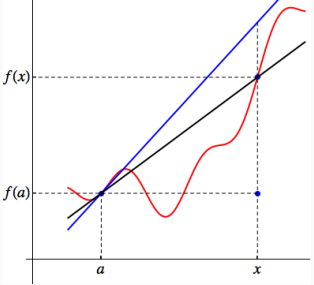
\includegraphics[scale=0.5]{rozdziały/images/Analiza/pochodna_interpretacja_shooter.png}
\end{figure}

\textbf{Iloraz różnicowy}
$$
\frac{f(x)-f(a)}{x-a} = tg \alpha 
$$
to tangens kąta $\alpha$ nachylenia sieczniej do osi OX.

W granicy, $f'(a)$ to współczynnik kierunkowy stycznej do wykresu f w punkcie $(a, f(a))$.

Prosta o równaniu $y-f(a)=f'(a)(x-a)$ jest styczna do wykresu f.

Naturalna interpretacja wskazuje, że znak pochodnej związany jest z monotonicznością. W szczególności, gdy mamy na wykresie "dołek" - ekstremum lokalne, styczna do funkcji w tym punkcie jest pozioma, tj. pochodna wynosi 0.

\begin{example}
    Pochodne funkcji elementarnych
    $$
    f(x)=const \Longrightarrow f'(x) = 0 \qquad (x^n)' = nx^{n-1} \qquad (\exp x)' = \exp x \qquad (\ln y)' = \frac{1}{y}, \ y > 0
    $$
    $$
    (\sin x)' = \cos x \qquad (\cos x)' = -\sin x \qquad (\tg x)' = 1 + \tg^2 x \qquad (\arctan x)' = \frac{1}{1+x^2}
    $$
    $$
    (ctg x)' = -1 - ctg^2x \qquad (\arcsin y)' = \frac{1}{\sqrt{1-y^2}} , \ -1 < y < 1
    $$
\end{example}

\subsection{Własności pochodnej}
Jeśli $f, g: \RR \supset A \to \RR$ są różniczkowalne w $a \in A$, to
\begin{itemize}
    \item $(f+g)'(a) = f'(a) + g'(a)$
    \item $(fg)'(a)=f'(a)g(a) + f(a)g'(a)$
    \item $\left(\frac{1}{g}\right)'(a)=-\frac{g'(a)}{g^2(a)}$ o ile $g(a)\neq 0$
    \item $(f \circ g )'(a) = f'(g(a))\cdot g'(a)$
    \item Jeśli $g=f^{-1}$, $g$ ciągła w punkcie $b=f(a)$, $f'(a)\neq 0$, to $g'(b)=\frac{1}{f'(a)}$
\end{itemize}

\textbf{Różniczkowalność} $\Longrightarrow$ \textbf{ciągłość}, ale nie na odwrót.

\textbf{Uwaga}:
Może być tak, że funkcja jest ciągła na całej swojej dziedzinie, ale nie jest różniczkowalna w żadnym punkcie ze swojej dziedziny. Przykładem takiej funkcji jest \href{https://pl.wikipedia.org/wiki/Funkcja_Weierstrassa}{funkcja Weierstrassa}.

% TODO
\begin{editorsnote}
    W części teoretycznej brak informacji o funkcjach klasy $C^n$, a pojawia się to w zadaniach i dalszej teorii.
\end{editorsnote}

\subsection{Reguła de l'Hospitala}
Reguła de l'Hospitala ułatwia obliczanie granic wyrażeń nieoznaczonych typu $\frac{0}{0}$ i $\frac{\infty}{\infty}$.

\textbf{Twierdzenie}: Załóżmy, że $f,g:\RR\supset P\to\RR$ są różniczkowalne w punkcie skupienia $a\in P$ zbioru $P\subset\RR$, a ponadto $f(a)=g(a)=0\neq g'(a)$. Wówczas granica
$$\lim_{x\to a}\frac{f(x)}{g(x)}$$
istnieje i jest równa $f'(a)/g'(a)$.

\begin{example}
    Policzymy granicę
    $$\lim_{x\to0}\frac{1+2x+x\sin{x}-x^2\cos{x}-(\exp{x})^2}{\sqrt{1+x^2}-\exp(x^2)}$$
    Wstawiając 0 w miejsce $x$ widzimy, że powyższa granica jest postaci $\frac{0}{0}$, więc używamy reguły de l'Hospitala:
    $$\lim_{x\to0}\frac{1+2x+x\sin{x}-x^2\cos{x}-(\exp{x})^2}{\sqrt{1+x^2}-\exp(x^2)}=\lim_{x\to0}\frac{0+2+\sin{x}+x\cos{x}-2x\cos{x}+x^2\sin{x}-2\exp(2x)}{2x\frac{1}{2\sqrt{1+x^2}}-2x\exp(x^2)}=$$
    $$=\lim_{x\to0}\frac{2+x^2\sin{x}+\sin{x}-x\cos{x}-2\exp(2x)}{\frac{x}{\sqrt{1+x^2}}-2x\exp(x^2)}=*$$
    Wstawiając 0 za $x$ widzimy, że ponownie uzyskujemy granicę postaci $\frac{0}{0}$, więc znów korzystamy z reguły de l'Hospitala:
    $$*=\lim_{x\to0}\frac{0+2x\sin{x}+x^2\cos{x}+\cos{x}-\cos{x}+x\sin{x}-2\cdot2\exp(2x)}{\frac{1\sqrt{1+x^2}-x\frac{2x}{2\sqrt{1+x^2}}}{1+x^2}-2\exp(x^2)-2x\cdot2x\exp(x^2)}=$$
    $$=\lim_{x\to0}\frac{3x\sin{x}+x^2\cos{x}-4\exp(2x)}{\frac{1+x^2-x^2}{(1+x^2)\sqrt{1+x^2}}-4x^2\exp(x^2)-2\exp(x^2)}=\frac{3\cdot0\sin{0}+0\cos{0}-4\exp(0)}{\frac{1}{(1+0)\sqrt{1+0}}-4\cdot0\exp(0)-2\exp(0)}=\frac{-4}{1-2}=4$$
    Reguła de l'Hospitala zawsze doprowadzi nas do wyniku, ale jak widać na przykładzie powyżej, czasami rachunki potrafią być długie i żmudne.
\end{example}

\begin{problems}
    \prob Dana jest funkcja $f: (a, b) \to \mathbb{R}$ różniczkowalna na $(a, x_0) \cup (x_0, b)$, gdzie $x_0 \in (a,b)$. Wynika z tego, że
    \answers{$f$ jest ciągła na $(a, b)$}{jeśli $f$ jest ciągła na $(a, b)$, to jest też różniczkowalna na $(a, b)$}{$f$ ma ograniczony zbiór wartości na każdym przedziale domkniętym zawartym w $(a, b)$}
    \prob Funkcja $f:\RR\longrightarrow\RR$ jest różniczkowalna oraz $f(0)=f(1)=0$. Wynika z tego, że skończona jest granica
    \answers{$\Limn nf\left(\frac{1}{n}\right)$}{$\Limn nf\left(\frac{n+1}{n}\right)$}{$\Limn nf\left(\frac{n}{n+1}\right)$}
    \prob Dla $a, b \in \RR$ funkcja $f_{a, b} : \RR \to \RR$ jest zdefiniowana wzorem
    \begin{equation*}
    f_{a, b}(x) =
        \begin{cases}
            e^x & \text{dla $x < 0$}\\
            ax + b & \text{dla $x \geq 0$}
        \end{cases}       
    \end{equation*}
    Wtedy
    \answers{istnieje dokładnie jedna para $a, b \in \RR$, taka że $f_{a, b}$ jest funkcją dwukrotnie różniczkowalną}{istnieje nieskończenie wiele par $a, b \in \RR$, takich że $f_{a, b}$ jest funkcją ciągłą}{istnieje dokładnie jedna para $a, b \in \RR$, taka że $f_{a, b}$ jest funkcją różniczkowalną}
    \prob Funkcja $f:(0;1) \to \RR$ zadana wzorem $f(x) = \sqrt{|\sin{x}|}$
    \answers{jest różniczkowalna}{jest ciągła i osiąga swój kres górny}{ma pochodną ograniczoną}
\end{problems}

\section{Twierdzenie Lagrange'a o wartości średniej}
\textbf{Twierdzenie}:
Załóżmy, że $a<b$, zaś funkcja $f:[a,b]\to\RR$ jest ciągła na $[a,b]$ i różniczkowalna w każdym punkcie $x\in(a,b)$. Wówczas istnieje taki punkt $\xi\in(a,b)$, że
$$f'(\xi)=\frac{f(b)-f(a)}{b-a}$$
Twierdzenie Lagrange'a ma bardzo prostą interpretację geometryczną: w przedziale $(a,b)$ istnieje taki punkt, w którym styczna do wykresu $f$ jest równoległa do siecznej, poprowadzonej przez dwa końce łuku wykresu.
\begin{figure}[h]
    \centering
    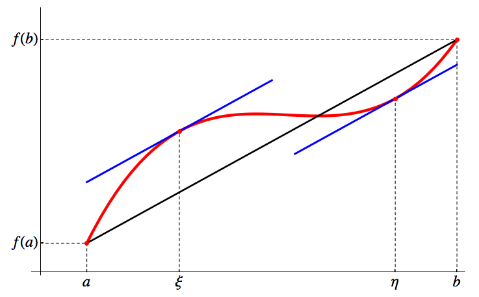
\includegraphics[scale=0.5]{rozdziały/images/Analiza/lagrange_interpretacja_geom.png}
\end{figure}

\textbf{Wniosek}: Załóżmy, że $A\subset\RR$, $[c,d]\subset A$, $c<d$, a funkcja $f:A\to\RR$ jest ciągła na $[c,d]$ i różniczkowalna w $(c,d)$. Zachodzą wówczas następujące implikacje:
\begin{itemize}
    \item Jeśli $f'(x)\geq0$ dla każdego $x\in(c,d)$, to $f$ jest niemalejąca na $[c,d]$
    \item Jeśli $f'(x)>0$ dla każdego $x\in(c,d)$, to $f$ jest rosnąca na $[c,d]$
    \item Jeśli $f'(x)<0$ dla każdego $x\in(c,d)$, to $f$ jest malejąca na $[c,d]$
    \item Jeśli $f'(x)\leq0$ dla każdego $x\in(c,d)$, to $f$ jest nierosnąca na $[c,d]$
\end{itemize}

\begin{exam}
    Funkcja $f : [0; 1] \rightarrow \RR$ jest różniczkowalna oraz $f(0) = 1, f(1) = 0$. Wynika z tego, że istnieje $x \in [0; 1]$, dla którego $f'(x)$ jest
    \answers
    {mniejsze od 0}
    {równe $-1$}
    {większe bądź równe 1}
    \bigskip

    \begin{enumerate}[\bf A.]
        \item Ponieważ funkcja zmalała między $0$ a $1$, to na jakimś odcinku na przedziale  $[0,1]$ pochodna była ujemna.

        \item Z twierdzenia Lagrange'a o wartości średniej dostajemy, że istnieje takie $\xi$, że $f'(\xi)=\frac{f(b)-f(a)}{b-a}=\frac{0-1}{1-0}=-1$, gdzie $a=0$, $b=1$.

        \item Nie możemy nic na ten temat założyć. Funkcja $f(x) = 1-x$ jest kontrargumentem.
    \end{enumerate}
\end{exam}

\subsection{Wypukłość}
Załóżmy, że $f:P=(a,b)\to\RR$ jest dwukrotnie różniczkowalna. Wówczas:
\begin{itemize}
    \item Jeśli $f''\geq0$ na $P$, to $f$ jest wypukła na $P$
    \item Jeśli $f''>0$ na $P$, to $f$ jest ściśle wypukła na $P$
    \item Jeśli $f''<0$ na $P$, to $f$ jest ściśle wklęsła na $P$
    \item Jeśli $f''\leq0$ na $P$, to $f$ jest wklęsła na $P$
\end{itemize}

\section{Wzór Taylora}
Oznaczmy $f^{(n)}$ jako $n$-tą pochodną funkcji $f$.

\textbf{Wzór Taylora z resztą Peano}:
Niech $P\subset\RR$ będzie przedziałem otwartym, $x_0\in P$. Załóżmy, że $f:P\to\RR$ ma $(k-1)$ pochodnych na $P$ i $k$-tą pochodną w punkcie $x_0$. Wówczas
$$\purple{f(x)=\sum_{j=0}^k\frac{f^{(j)}(x_0)}{j!}(x-x_0)^j+r(x)},\quad\lim_{x\to x_o}\frac{r(x)}{(x-x_0)^k}=0$$

\textbf{Wzór Taylora z resztą Lagrange'a}:
Załóżmy, że funkcja $f:(a,b)\to\RR$ ma w przedziale $(a,b)$ pochodne do rzędu $(k+1)$ włącznie. Wówczas, dla każdego $x_0\in(a,b)$ i każdego $x\in(a,b)$ istnieje taki punkt $c$, pośredni między $x_0$ i $x$, że
$$\purple{f(x)=\sum_{j=0}^k\frac{f^{(j)}(x_0)}{j!}(x-x_0)^j + \frac{f^{(k+1)}(c)}{(k+1)!}(x-x_0)^{k+1}}$$

\begin{example}
    Rozwinięcie znanych funkcji w szereg Taylora:
    $$\purple{\exp(x)=\sum_{n=0}^\infty\frac{x^n}{n!}} = 1+\frac{1}{1!}x+\frac{1}{2!}x^2+\frac{1}{3!}x^3+\cdots$$
    $$\purple{\sin(x)=\sum_{n=0}^\infty\frac{(-1)^n}{(2n+1)!}x^{2n+1}} = x-\frac{x^3}{3!}+\frac{x^5}{5!}-\frac{x^7}{7!}+\cdots$$
    $$\purple{\cos(x)=\sum_{n=0}^\infty\frac{(-1)^n}{(2n)!}x^{2n}} = 1-\frac{x^2}{2!}+\frac{x^4}{4!}-\frac{x^6}{6!}+\cdots$$
    $$\purple{\ln(1+x)=\sum_{n=1}^\infty(-1)^{n+1}\frac{x^n}{n}} = x-\frac{x^2}{2}+\frac{x^3}{3}-\frac{x^4}{4}+\cdots$$
\end{example}

\subsection{Szeregi potęgowe}
\textbf{Definicja} $\limsup$:
$$\limsup_{n\to\infty}a_n = \inf_{n\in\NN}\left(\sup_{k\geq n}a_k\right) = \lim_{n\to\infty}s_n, \quad\text{gdzie}\quad s_n = \sup_{k\geq n}a_k$$
Równoważne definicje:
\begin{itemize}
    \item Kres górny zbioru granic wszystkich podciągów $(a_n)$
    \item Największa spośród granic podciągów $(a_n)$
\end{itemize}

Szereg potęgowy o współczynnikach $a_n\in\CC$ i środku $z_0\in\CC$:
$$\purple{S(z)=\sum_{n=0}^\infty a_n(z-z_0)^n}$$

\textbf{Twierdzenie}:
Szereg jw. jest zbieżny (bezwzględnie) w kole $|z-z_0|<R$ i rozbieżny dla $|z-z_0|>R$, gdzie
$$\purple{\frac{1}{R}=\limsup_{n\to\infty}\sqrt[n]{|a_n|}}$$
\textbf{Uwaga}: na brzegu koła zbieżności, dla $|z-z_0|=R$, może być różnie \ldots

\begin{example}
    Pokażemy, że szereg $\sin(x)=\sum_{k=0}^\infty\frac{(-1)^k}{(2k+1)!}x^{2k+1}$ ma promień zbieżności $R=\infty$. Zauważmy, że dla $n$ parzystych mamy $a_n=0$. Dla $n$ nieparzystych dostajemy podciąg ciągu $(n!)^{-1/n}$, który zbiega do 0:
    $$
    \limsup_{n\to\infty}|a_n|^{1/n} = \limsup_{n\to\infty}\left|\frac{1}{(n!)^{1/n}}\right| = \Limn\frac{1}{(n!)^{1/n}} = 0,
    $$
    a więc $\frac{1}{R}=0 \Rightarrow R = \infty$.
\end{example}

\subsection{Różniczkowalność sumy szeregu potęgowego}
\textbf{Twierdzenie}:
Załóżmy, że $R>0$ jest promieniem zbieżności szeregu potęgowego $S(z)=\sum_{n=0}^\infty a_nz^n$. Wtedy funkcja $S$ ma pochodną w każdym punkcie $z\in\{w\in\CC:|w|<R\}$ i zachodzi wzór
$$\purple{S'(z)=\sum_{n=1}^\infty na_nz^{n-1}}$$

\textbf{Wniosek}:
\begin{itemize}
    \item Suma szeregu potęgowego jest ciągła wewnątrz koła zbieżności
    \item Suma szeregu potęgowego jest $C^\infty$ wewnątrz koła zbieżności
    \item Dla $k\in\NN$ jest $$S^{(k)}(z)=\sum_{n=k}^\infty n(n-1)\ldots(n-k+1)a_nz^{n-k},\quad S^{(k)}(0) = k!\cdot a_k$$
    (każdy szereg potęgowy sam jest swoim szeregiem Tayolora)
\end{itemize}

\begin{problems}
    \prob Dany jest szereg $S(x) = \sum_{n = 2}^{\infty} a_n x^n$ zbieżny dla $x \in (-1, 1)$ oraz rozbieżny w $x = -1$. Wynika z tego, że
    \answers{$S(x)$ jest rozbieżny w $x = 1$}{$S(x)$ jest rozbieżny w $x = -2$}{$S(x)$ jest różniczkowalny na odcinku $(-1, 1)$ oraz $S'(0) = 0$}
    \prob Niech $f: \mathbb{R} \to \mathbb{R}$ będzie dana wzorem $f(x) = \left|-3x+x^2-5\right|$. Prawdą jest, że
    \answers{$f$ jest różniczkowalna}{$f$ jest dwukrotnie różniczkowalna}{jej pierwszy szereg Taylora w otoczeniu $x_0 = 0$ i $x = 1$ wynosi $\sqrt{2}$}
    \prob Niech $f: [0, 1] \to \mathbb{R}$ będzie ciągła. Wtedy
    \answers{$f'(x)$ istnieje dla każdego $x \in ([0, 1] \setminus A)$ gdzie $A$ jest pewnym skończonym podzbiorem $\mathbb{R}$}{zbiór wartości $f$ jest punktem lub przedziałem domkniętym}{$f$ jest sumą pewnego szeregu potęgowego}
    \prob Niech $H_n := \sum_{j=1}^n \frac{1}{j}$ będzie $n$-tą liczbą harmoniczną. Wówczas
    \answers{promień zbieżności szeregu potęgowego $\sum_{n=1}^{\infty} H_n x^n $ wynosi 1}{$\Limn \frac{H_n}{\ln n} = 1$}{$\Limn (H_n - \ln n) = 0$}
\end{problems}

\section{Zbieżność ciągów liczbowych i funkcyjnych}
Powiemy, że ciąg funkcji $(f_n)$ jest \textbf{zbieżny punktowo} do $f$ na zbiorze $X$ wtedy i tylko wtedy, gdy dla każdego punktu $x\in X$ zachodzi równość
$$\purple{f(x) = \lim_{n\to\infty}f_n(x)}$$
Piszemy wtedy: $f_n\to f$ na $X$.

Powiemy, że ciąg funkcji $(f_n)$ jest \textbf{zbieżny jednostajnie} do $f$ na zbiorze $X$ wtedy i tylko wtedy, gdy zachodzi warunek: dla każdego $\epsilon>0$ istnieje $n_0=n_0(\epsilon)\in\NN$ takie, że dla wszystkich $x\in X$ i wszystkich $n>n_0$ jest
$$\purple{|f(x)-f_n(x)|<\epsilon}$$
Piszemy wtedy: $f_n\toto f$ na $X$.

\textbf{Twierdzenie}:
Załóżmy, że $P\subset\RR$ jest dowolnym przedziałem. Niech $f_n:P\to\RR$ będą funkcjami ciągłymi na $P$. Jeśli $f_n\toto f$ na $P$, to $f$ jest ciągła na $P$.

Mówimy, że szereg funkcji $\sum_{k=1}^\infty f_k(x)$ jest zbieżny punktowo (jednostajnie) do funkcji $f(x)$ na zbiorze $X$ wtedy i tylko wtedy, gdy ciąg sum częściowych $S_n=\sum_{k=1}^n f_k$ tego szeregu jest zbieżny do $f$ punktowo (jednostajnie) na zbiorze $X$.

\begin{example}
    Niech $f_n:[0,1]\to\RR$ będzie dana wzorem $f_n(x)=x^n$. Wtedy
    $$
    \Limn f_n(x) = \Limn x^n = f(x) := \begin{cases}
        0, & x\in[0,1) \\
        1, & x = 1
    \end{cases}
    $$
    Innymi słowy, ciąg $f_n$ jest zbieżny \textbf{punktowo} na $[0,1]$ do funkcji $f$. NIE jest jednak zbieżny \textbf{jednostajnie}: dla każdego $n\in\NN$ jest
    $$
    |f_n(2^{-1/n}) - f(2^{-1/n})| = \frac{1}{2} - 0 = \frac{1}{2},
    $$
    a zatem warunek z definicji zbieżności jednostajnej nie zachodzi dla żadnej liczby $\epsilon<\frac{1}{2}$.
\end{example}

\subsection{Kryteria zbieżności jednostajnej}
\textbf{Twierdzenie}:
Niech $f_n:X\to\RR$ dla $n=1,2,\ldots$. Następujące warunki są równoważne:
\begin{itemize}
    \item Ciąg $(f_n)$ jest zbieżny jednostajnie na $X$ do pewnej funkcji $f:X\to\RR$
    \item Ciąg $(f_n)$ spełnia \textbf{jednostajny warunek Cauchy'ego}: dla każdego $\epsilon>0$ istnieje $n_0\in\NN$ takie, że dla wszystkich $m,n>n_0$ i wszystkich $x\in X$ zachodzi nierówność
    $$\purple{|f_n(x)-f_m(x)|<\epsilon}$$
\end{itemize}

\textbf{Twierdzenie (Kryterium Weierstrassa)}:
Niech $f_n:X\to\RR$ dla $n=1,2,\ldots$. Jeśli $|f_n(x)|\leq a_n$ dla $n\in\NN$, a szereg liczbowy $\sum_{n=1}^\infty a_n$ jest zbieżny, to wówczas szeregi funkcyjne $\sum_{n=1}^\infty f_n(x)$ oraz $\sum_{n=1}^\infty |f_n(x)|$ są zbieżne jednostajnie na $X$. W takiej sytuacji mówimy, że szereg $\sum f_n(x)$ jest zbieżny jednostajnie i bezwzględnie.

\subsection{Różniczkowanie ciągów funkcyjnych}
\textbf{Twierdzenie}:
Niech $f_n:\RR\supset[a,b]\to\RR$ będą różniczkowalne. Jeśli ciąg $f_n'\toto g$ na $[a,b]$, a ponadto istnieje taki punkt $x_0\in[a,b]$, że ciąg $(f_n(x_0))$ jest zbieżny, to wówczas
\begin{itemize}
    \item $f_n\toto f$ na $[a,b]$, gdzie $f$ ciągła
    \item Funkcja $f$ jest różniczkowalna na $[a,b]$ i $f'=g$
\end{itemize}

\begin{problems}
    \prob Funkcja $f:\RR\rightarrow\RR$ jest zadana wzorem $f(x)=\sum_{n=1}^\infty\frac{\sin(nx)}{n^3}$. Wynika z tego, że
    \answers{funkcja $f$ jest ograniczona na $\RR$}{funkcja $f$ jest różniczkowalna na $\RR$}{spełniona jest nierówność $16>f'(0)>\frac{1}{16}$}
    \prob Ciąg funkcji $f_n(x) = x^n$ jest
    \answers{zbieżny punktowo na $[0, 1]$}{zbieżny jednostajnie na $[0, 1)$}{ograniczony na $[0, 1 + \epsilon)$ dla pewnego $\epsilon > 0$}
    \prob Ciąg funkcyjny $\{f_n\}_{n\geq1}$ składa się z funkcji $f_n : \RR \rightarrow \RR$ zdefiniowanych wzorami $f_n(x) = x - \frac{1}{n}$ dla $x \in \RR$. Ten ciąg funkcyjny jest
    \answers
    {zbieżny punktowo i jednostajnie}
    {niemal jednostajnie zbieżny}
    {zbieżny punktowo do funkcji ciągłej}
\end{problems}

\section{Ekstrema funkcji}
Niech $f:I\to\RR$, gdzie $I$ jest przedziałem w $\RR$. Mówimy, że funkcja $f$ ma w punkcie $a\in I$ maksimum lokalne (odpowiednio: minimum lokalne), jeśli istnieje taka liczba $\delta>0$, że dla wszystkich $x\in I$, $|x-a|<\delta$, zachodzi nierówność $f(a)\geq f(x)$ (odpowiednio: $f(a)\leq f(x)$).

Słowo \textbf{ekstremum} jest wspólną nazwą minimum i maksimum. Należy pamiętać, że wartość funkcji w punkcie ekstremum lokalnego nie musi być najmniejszą ani największą wartością funkcji na danym przedziale. Ekstremów może być wiele, a ponadto jeśli przedział jest otwarty, to funkcja w ogóle nie musi przyjmować swoich kresów.

\subsection{Warunki istnienia ekstremów}
\textbf{Lemat (Fermata, warunek konieczny)}:
Jeśli $I$ jest odcinkiem otwartym, $a\in I$, $f:I\to\RR$ jest różniczkowalna w punkcie $a$ i $f$ ma w $a$ ekstremum lokalne, to $f'(a)=0$.

Interpretacja geometryczna: styczna do wykresu funkcji różniczkowalnej w punkcie ekstremum lokalnego jest pozioma.

\begin{example}
    Należy pamiętać, że warunek ten \underline{nie} jest wystarczający, a najlepszym na to przykładem jest funkcja $f(x)=x^3$. Jej pochodna $f'(x)=3x^2$ zeruje się w $x_0=0$, ale oczywiście $f$ nie ma w tym punkcie ekstremum, co widać na wykresie.
\end{example}

\textbf{Twierdzenie (Rolle’a)}:
Załóżmy, że $a<b$, zaś funkcja $f:[a,b]\to\RR$ jest ciągła na $[a,b]$ i różniczkowalna w każdym punkcie $x\in(a,b)$. Jeśli $f(a)=f(b)$, to istnieje taki punkt $x_0\in(a,b)$, że $f'(x_0)=0$.

\textbf{Warunek dostateczny istnienia ekstremum}:
Funkcja ciągła $f:[a,b]\to\RR$, różniczkowalna w $(a,b)$ ma w punkcie $x_0\in(a,b)$:
\begin{itemize}
    \item maksimum lokalne wtedy i tylko wtedy, gdy $f'(x_0)=0$ oraz istnieje $\delta>0$ takie, że $f'(x)>0$ dla $x\in(x_0-\delta, x_0)$ i $f'(x)<0$ dla $x\in(x_0, x_0+\delta)$;
    \item minimum lokalne wtedy i tylko wtedy, gdy $f'(x_0)=0$ oraz istnieje $\delta>0$ takie, że $f'(x)<0$ dla $x\in(x_0-\delta, x_0)$ i $f'(x)>0$ dla $x\in(x_0, x_0+\delta)$.
\end{itemize}

\begin{exam}
    Liczba rozwiązań równania $e^x = 2x$ jest równa
    \answers{0}{1}{2}
    Oznaczmy $f(x)=e^x-2x$. Wtedy $f'(x)=e^x-2$. Policzmy ekstremum funkcji $f$. Warunek konieczny: $f'(x_0)=0 \Rightarrow x_0=\ln{2}$. Zauważmy, że dla $x<x_0$ jest $f'(x)<0$ oraz dla $x>x_0$ jest $f'(x)>0$. Z warunku dostatecznego otrzymujemy, że $x_0$ jest minimum lokalnym funkcji $f$. Skoro $f(x_0)=e^{\ln{2}}-2\ln{2}=2-2\ln{2}>2-2\ln{e}=0$, to znaczy, że $f$ nie ma miejsc zerowych, bo jest dodatnia w całej swojej dziedzinie. Tak więc, liczba rozwiązań równania $e^x=2x$ wynosi 0.
\end{exam}

\begin{problems}
    \prob Dana jest różniczkowalna funkcja $f: \RR \to \RR$, taka że $f'(0) = 0$. Wynika z tego, że
    \answers{$f$ ma ekstremum lokalne w $x = 0$}{jeśli dla każdego $x \neq 0$ zachodzi $f'(x) < 0$, to $f$ jest malejąca}{$f$ jest ciągła w $x = 2019$}
\end{problems}

\section{Całki}
$F$ jest funkcją pierwotną $f$ na $P$, gdy $F'=f$ na $P$.

\subsection{Całka nieoznaczona}
Niech $f:P\to\RR$, gdzie $P\subset\RR$ jest dowolnym przedziałem. Całką nieoznaczoną funkcji $f$ nazywamy rodzinę wszystkich funkcji pierwotnych funkcji $f$. Używa się zwykle zapisu
$$
\purple{\int f(x)\ dx = F(x) + const},
$$
gdzie $F$ jest dowolnie wybraną funkcją pierwotną $f$ na danym przedziale.

\begin{example}
    Najważniejsze wzory na całki nieoznaczone:
    $$\int x^n\ dx = \frac{1}{n+1}x^{n+1} + C, \quad n\neq -1 \qquad \int\frac{1}{x}\ dx = \ln|x| + C \qquad \int a^x\ dx = \frac{a^x}{\ln{a}} + C$$
    $$\int e^x\ dx = e^x + C \qquad \int\sin{x}\ dx = -\cos{x} + C \qquad \int\cos{x}\ dx = \sin{x} + C$$
    $$\int \tg{x}\ dx = -\ln|\cos{x}| + C \qquad \int \ctg{x}\ dx = \ln|\sin{x}| + C \qquad \int\frac{1}{\cos^2{x}}\ dx = \tg{x} + C$$
    $$\int\frac{1}{\sin^2{x}}\ dx = -\ctg{x} + C \qquad \int\frac{1}{1+x^2}\ dx = \arctg{x} + C \int\frac{1}{\sqrt{1-x^2}}\ dx = \arcsin{x} + C$$
\end{example}

\subsection{Własności całek nieoznaczonych}
\textbf{Liniowość całki}:
Jeśli $f,g:P\to\RR$ są ciągłe, zaś $a,b\in\RR$, to
$$\purple{\int(af(x)+bg(x))\ dx = a\int f(x)\ dx + b\int g(x)\ dx}$$
Dowód: przez wzór na pochodną sumy.

\textbf{Całkowanie przez części}:
Jeśli $f,g:P\to\RR$ są różniczkowalne, to
$$\purple{\int f(x)\cdot g'(x)\ dx = f(x)g(x) - \int f'(x)\cdot g(x)\ dx}$$
Dowód: przez wzór na pochodną iloczynu.

\begin{example}
    Policzymy całkę $\int\ln{x}\ dx$. Połóżmy $f(x)=\ln{x}$ i $g'(x)=1$. Wtedy $f'(x)=\frac{1}{x}$ oraz $g(x)=x$. Stosując powyższy wzór dla $f$ i $g$ zdefiniowanych przed chwilą, dostajemy:
    $$
    \int\ln{x}\ dx = x\ln{x} - \int\frac{1}{x}\cdot x\ dx = x\ln{x} - \int dx = x\ln{x} - x + C
    $$
\end{example}

\textbf{Całkowanie przez podstawienie}:
Niech $f,g'$ będą ciągłe i niech $F$ będzie funkcją pierwotną $f$. Wtedy
$$\purple{\int f(g(x))g'(x)\ dx = F(g(x) + C}$$
Dowód: przez wzór na pochodną złożenia.

\begin{example}
    Policzymy całkę $\int\sin^5{x}\cos{x}\ dx$. Podstawimy $t=\sin{x}$. Wtedy $dt=\cos{x}\ dx$. Dostajemy
    $$
    \int\sin^5{x}\cos{x}\ dx = \int t^5\ dt = \frac{t^6}{6} + C = \frac{\sin^6{x}}{6} + C
    $$
    Intuicja: szukamy takiego podstawienia, że mając $t=p(x)$, gdzieś pod całką jest czynnik $p'(x)\cdot dx$, co fajnie działa np. w przypadku iloczynu sinusa z cosinusem, jak widać powyżej.
\end{example}

\subsection{Całka oznaczona}
Niech $f:[a,b]\to\RR$ będzie funkcją ciągłą. Całką oznaczoną funkcji $f$ na przedziale $[a,b]$ nazywamy liczbę
$$
\purple{\int_a^b f(x)\ dx = F(b) - F(a)},
$$
gdzie $F$ jest dowolną funkcją pierwotną funkcji $f$.

Wszystkie własności całki nieoznaczonej mają tu zastosowanie. Generalnie, jeśli chcemy policzyć całkę oznaczoną, to liczymy całkę nieoznaczoną, a następnie podstawiamy krańce przedziałów za $x$ i odejmujemy od siebie.

\subsection{Interpretacja geometryczna}
Całkę możemy interpretować jako pole pod wykresem funkcji. Suma $\sum_{i=1}^n f(t_i)(x_i-x_{i-1})$ to suma pól prostokątów. Dla dużych $n$, gdy podstawy wszystkich prostokątów są małe, wartość tej sumy jest dobrym przybliżeniem całki $\int_a^b f(x)\ dx$, tzn. pola zacieniowanego obszaru.
\begin{figure}[ht]
    \centering
    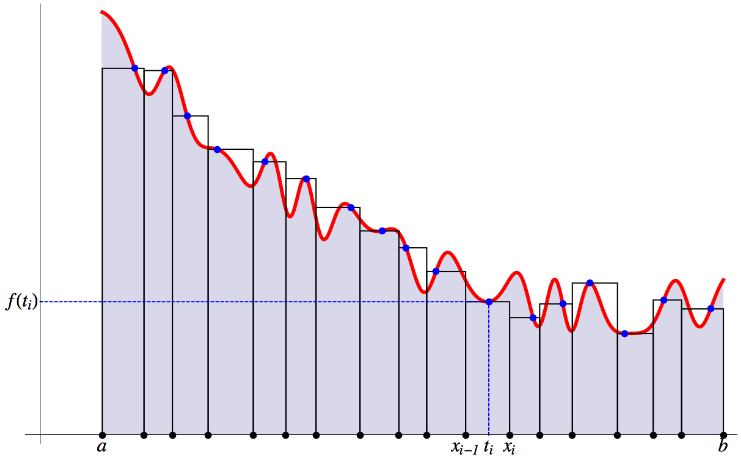
\includegraphics[scale=0.5]{rozdziały/images/Analiza/calka_interpretacja_geom.png}
\end{figure}

\subsection{Całka niewłaściwa}
Załóżmy, że funkcja $f:[a,\infty)\to\RR$ jest ciągła. Jeśli istnieje skończona granica
$$
\lim_{y\to\infty}\int_a^y f(x)\ dx,
$$
to nazywamy ją całką niewłaściwą funkcji $f$ na przedziale $[a,\infty)$ i oznaczamy
$$
\int_a^\infty f(x)\ dx
$$
Mówimy wtedy, że całka niewłaściwa $f$ na $[a,\infty)$ jest zbieżna. Jeśli granica nie istnieje, to mówimy, że całka $\int_a^\infty f(x)\ dx$ jest rozbieżna. Analogicznie definiujemy całkę niewłaściwą funkcji $f:(-\infty, a]\to\RR$.

\begin{example}
    Policzymy całkę $\int_0^\infty e^{-x}\ dx$. Mamy
    $$
    \int_0^\infty e^{-x}\ dx = \lim_{y\to\infty} \int_0^y e^{-x}\ dx = \lim_{y\to\infty} -e^{-x}\Big|_0^y = \lim_{y\to\infty} (-e^{-y} + e^0) = \lim_{y\to\infty} (1-e^{-y}) = 1,
    $$
    tak więc całka $\int_0^\infty e^{-x}\ dx$ jest zbieżna do 1.
\end{example}

\begin{problems}
    \prob Niech $\{f_n\}_{n \geq 0}$ będzie ciągiem ograniczonych funkcji typu $(0, 1) \to \mathbb{R}$, takich że $\int_0^1{f_n(t) \dt} = 0$. Wtedy
    \answers{istnieje prawostronna granica $f_0$ w $0^+$}{$\{f_n(x)\}_{n \geq 0}$ jest zbieżny do $0$ dla każdego $x \in (0, 1)$}{jeśli $\{f_n(x)\}_{n \geq 0}$ jest zbieżny do $0$ dla każdego $x \in (0, 1)$, to $\left\{\int_0^1{|f_n(t)| \dt}\right\}_{n \geq 0}$ jest zbieżny do $0$}
    \prob Niech $f : (-1, 1) \to \RR$ będzie zdefiniowana wzorem
    $$f(x) = \frac{1}{x^2 - 4x + 3}$$
    Wtedy
    \answers{funkcja $f$ jest ograniczona na $(-1, 1)$}{pochodna $f^{(1000)}(0)$ wynosi $1000!\left(\frac{1}{2} - \frac{1}{6 \cdot 3^{1000}}\right)$}{zachodzi $\int_{-1}^{0} f(t) \dt = \frac{\ln{3} - \ln{2}}{2}$}
\end{problems}

\section{Elementy teorii miary}

% TODO
\begin{editorsnote}
    Rozdział nie jest jeszcze stworzony -- w historii przeanalizowanych na potrzeby tego repetytorium egzaminów pojawiło się tylko jedno zadanie z teorii miary, w dodatku w miarę proste.
\end{editorsnote}

\begin{problems}
    \prob W pewnej metryce $\rho$ zachodzi $\rho(x_1, x_2) = 7$. Dane są dwie otwarte kule, $K_1$ o środku $x_1$ i promieniu 1 oraz $K_2$ o środku w $x_2$ i promieniu 2. Wtedy
    \answers
    {$(K_2 \cup K_1)$ jest zbiorem otwartym}
    {istnieje kula otwarta o promieniu $8$ zawierająca kulę $K_1$ i $K_2$}
    {zbiór $(K_1 \cap K_2)$ jest niepusty}
\end{problems}

\begin{solutions}
    \sol Jeśli ciąg liczb rzeczywistych dodatnich $a_n$ jest monotoniczny i ograniczony, to
    \answerss{ciąg $\sin (a_n)$ jest monotoniczny}{ciąg $\cos (a_n)$ jest zbieżny}{ciąg $\log (a_n)$ jest ograniczony}{NIE}{TAK}{NIE}
    Ciąg $a_n$ jest zbieżny. \textbf{A.} Nie musi tak wcale być, np dla ciągu $a_1=\frac{\pi}{2}, a_2=\frac{-3\pi}{2}, a_n=\frac{1}{n}$ dla $n> 2$. \textbf{B.} jest zbieżny, bo $\lim_{n\to\infty}cos(a_n)=cos\left(\lim_{n\to\infty}a_n\right)$. \textbf{C.} dla $a_n=\frac{1}{n}$ mamy granicę równą $0$ a $\lim_{n\to 0}log(n) = -\infty$.
    
    % Grześ
    \sol Ciąg, którego $n$-ty wyraz zadany jest wzorem $\cfrac{2010^n - n^{2010}}{2^{n^2}-2010^n}$,
    \answerss
    {jest zbieżny}
    {ma granicę równą $-1$}
    {ma granicę równą 0}
    {TAK}{NIE}{TAK}
    $$
    \lim_{n\to\infty}\frac{2010^n - n^{2010}}{2^{n^2}-2010^n} = \lim_{n\to\infty}\frac{1 - \frac{n^{2010}}{2010^n}}{\frac{2^{n^2}}{2010^n}-1} = \lim_{n\to\infty}\frac{1 - \frac{n^{2010}}{2010^n}}{(\frac{2^{n}}{2010})^n-1}
    $$
    Funkcja wykładnicza rośnie szybciej niż wielomianowa, więc składnik $\frac{n^{2010}}{2010^n}\to0$, a oczywiście $\frac{2^n}{2010}\to\infty$, więc $\lim_{n\to\infty}\frac{2010^n - n^{2010}}{2^{n^2}-2010^n}=\frac{1-0}{\infty-1}=0$. Ciąg jest zbieżny do 0, więc odpowiedzi \textbf{A} i \textbf{C} są prawdziwe.
    
    \sol Niech $\{a_n\}_{n \geq 0}$ będzie ograniczonym ciągiem dodatnich liczb rzeczywistych. Wtedy
    \answerss{jeśli $\{\sin(a_n)\}_{n \geq 0}$ jest zbieżny, to $a_n$ jest monotoniczny}{$\{\exp(-a_n)\}_{n \geq 0}$ posiada podciąg zbieżny do granicy dodatniej}{jeśli $\{\exp(-a_n)\}_{n \geq 0}$ jest zbieżny, to $\{\arctan(a_n)\}_{n \geq 0}$ ma granicę dodatnią}{NIE}{TAK}{NIE}
    \textbf{A.} podobnie jak w 1.1.A, nie musi tak być. \textbf{B.} $a_n$ jest ograniczony, więc posiada podciąg zbieżny. W takim razie ciąg $1/e^{a_n}$ ma podciąg zbieżny do granicy dodatniej. Wystarczy wziąć ten podciąg zbieżny z $a_n$ i wziąć z niego funkcję $\exp$. \textbf{C.} Niech $a_n=\frac{1}{n}$. Wtedy $\exp(-a_n)$ jest zbieżny, $a_n$ ograniczony, ale $arctan(a_n)$ zbiega do $arctan(0)=0$.
    
    % Grześ
    \sol Ciąg określony dla $n \geq 1$ wzorem $(1+\frac{1}{4^n})^{2^n}$ jest
    \answerss{zbieżny do 1}{rosnący, począwszy od pewnego miejsca}{ograniczony}{TAK}{NIE}{TAK}
    $$
    \lim_{n\to\infty}\left(1+\frac{1}{4^n}\right)^{2^n} = \lim_{n\to\infty}\left(\left(1+\frac{1}{4^n}\right)^{4^n}\right)^\frac{1}{2^n} = e^{\lim_{n\to\infty}\frac{1}{2^n}} = e^0 = 1
    $$
    Ciąg zbiega do 1, więc jest ograniczony. Odpowiedzi \textbf{A} i \textbf{C} są więc prawdziwe. Sprawdźmy, czy ciąg rośnie od pewnego miejsca. W tym celu sprawdzimy, czy iloraz $\frac{a_{n+1}}{a_n}>1$. Mamy
    $$
    \frac{a_{n+1}}{a_n} = \frac{(1+\frac{1}{4^{n+1}})^{2^{n+1}}}{(1+\frac{1}{4^n})^{2^n}} = \left(\frac{(1+\frac{1}{4^{n+1}})^2}{1+\frac{1}{4^n}}\right)^{2^n} = \left(\frac{1+\frac{2}{4^{n+1}}+\frac{1}{4^{2n+2}}}{1+\frac{1}{4^n}}\right)^{2^n}
    $$
    Musi być $1+\frac{2}{4^{n+1}}+\frac{1}{4^{2n+2}}>1+\frac{1}{4^n}$, czyli $\frac{2}{4}+\frac{1}{4^{n+2}}>1$, co jest równoważne $4^{n+2} < 2$. To jest oczywiście nieprawda dla dużych $n$, więc odpowiedź w \textbf{B} to \texttt{NIE}.
    
    % Grześ
    \sol Ciąg $a_n = \left(0.999 + \frac{1}{4n}\right)^{4n}$
    \answerss{jest zbieżny do liczby większej od 0}{jest zbieżny do liczby niewymiernej}{jest ograniczony z góry}{NIE}{NIE}{TAK}
    Możemy ograniczyć ciąg z dołu przez 0, bo wszystkie jego wyrazy są dodatnie. Zauważmy teraz, że dla bardzo dużych $n$ możemy ograniczyć go z góry $\left(0.999 + \frac{1}{4n}\right)^{4n}<\left(0.999 + 0.0001\right)^{4n}=\left(0.9991\right)^{4n}\to0$, bo podnosimy liczbę mniejszą od 1 do bardzo dużej potęgi. Z twierdzenia o trzech ciągach otrzymujemy $a_n\to0$, więc odpowiedzi \textbf{A} i \textbf{B} są fałszywe. Ograniczenie z góry możemy łatwo pokazać, np. $\left(0.999 + \frac{1}{4n}\right)^{4n} < \left(1 + \frac{1}{4n}\right)^{4n} \to e$, więc odpowiedź \textbf{C} jest prawdziwa.
    
    \sol $\{S_n\}_{n\geq1}$ jest ciągiem sum częściowych szeregu rozbieżnego. Wynika z tego, że ciąg $\{S_{n+1} - S_n\}_{n\geq1}$ jest
    \answerss
    {rozbieżny}
    {nieograniczony}
    {niezbieżny do 0}
    {NIE}{NIE}{NIE}
    Trzeba się dokładnie wczytać co jest ciągiem a co szeregiem. $S_n$ jest ciągiem, tak samo $S_{n+1} - S_n$. Powiedzmy, że szeregiem w zadaniu jest $\sum\frac{1}{n}$. Wtedy $S_n=1+\frac{1}{2} + \dots + \frac{1}{n}$, a $(S_{n+1}-S_n)= S_n + \frac{1}{n+1} - S_n=\frac{1}{n+1}$. Ten ciąg jest zbieżny do $0$, także ograniczony i nie rozbieżny.
    
    \sol Rozważmy szeregi:
    $$
    (A)\ \sum_{n=1}^{\infty}\frac{7^n+n^9+\ln(19^{n^2}+8)}{8^n-11^{\ln(1+n)}+2}\quad\text{oraz}\quad (B)\ \sum_{n=1}^{\infty}\frac{8^n-11^{\ln(1+n)}+2}{7^n+n^9+\ln(19^{n^2}+8)}
    $$
    \answerss{ciąg sum częściowych każdego z tych szeregów jest ograniczony}{szereg $(A)$ jest zbieżny}{szereg $(B)$ jest zbieżny}{NIE}{TAK}{NIE}
    
    Bystry czytelnik zauważy, że wyrazy $7^n$ i $8^n$ dominują w obydwu szeregach, więc przy liczeniu warunku koniecznego dostajemy:
    $\lim_{n\to\infty}\frac{7^n}{8^n}=0$ w szeregu $(A)$ oraz $\lim_{n\to\infty}\frac{8^n}{7^n}=\infty$ w szeregu $(B)$. Wynika z tego, że tylko szereg $(A)$ jest zbieżny, czyli ma ograniczony ciąg sum częściowych.
    
    \sol Funkcja $\textit{f}: \mathbb{R} \xrightarrow{} \mathbb{R}$ dana wzorem $f(x) = e^{-x^2} \cdot \sqrt[3]{x} \cdot \sin(e^{x^2})$
    \answerss{jest różniczkowalna na $\mathbb{R}$}{jest jednostajnie ciągła na $\mathbb{R}$}{spełnia warunek Lipschitza na $\mathbb{R}$}{NIE}{TAK}{NIE}
    \textbf{A.} Wywala się w 0. Aby to zobaczyć, policzmy pochodną w 0 z definicji:
    $$
    \lim_{x\to0}\frac{f(x)-f(0)}{x-0} = \lim_{x\to0}\frac{e^{-x^2}\cdot\sqrt[3]{x}\cdot\sin(e^{x^2})}{x} = \lim_{x\to0}\frac{e^{-x^2}\cdot\sin(e^{x^2})}{\sqrt[3]{x^2}} = \frac{e^0\cdot\sin(e^0)}{0} = \infty,
    $$
    czyli granica nie istnieje, a więc funkcja nie jest różniczkowalna w $\RR$, bo nie jest różniczkowalna w 0.

    \textbf{B.} Zbadajmy jednostajną ciągłość $g(x)=e^{-x^2}$. Z twierdzenia Lagrange'a o wartości średniej (o którym później) mamy, że jeśli $x<y$, to istnieje takie $c\in(x,y)$, że $g(y)-g(x)=(y-x)g'(c)=(y-x)(-2ce^{-c^2})$. Znając nierówność $e^x\geq x+1$ oraz $|x|^2+1\geq 2|x|$ nakładamy moduł na obydwie strony równości dostając:
    $$
    |g(y)-g(x)| = |y-x|\frac{2|c|}{e^{c^2}} \leq |y-x|\frac{2|c|}{c^2+1} \leq |y-x|\frac{2|c|}{2|c|} = |y-x|.
    $$
    Dostaliśmy oszacowanie $|g(x)-g(y)|\leq|x-y|$ dla dowolnych $x,y$. Znaczy to, że $g$ spełnia warunek Lipschitza ze stałą $L=1$, więc jest jednostajnie ciągła. Zadanie dla Czytelnika: pokazać, że przemnożenie $g$ przez $\sqrt[3]{x}\cdot\sin(e^{-x^2}$ nie popsuje jedostajnej ciągłości.

    \textbf{C.} Nie spełnia, bo jeśli położymy $y=0$ w nierówności z warunku Lipschitza, to dostaniemy $\big|\frac{f(x)}{x}\big|\leq L$. Z podpunktu \textbf{A.} wiemy, że nie da się tego ograniczyć dla małych $x$.

    %  Tomek
    \sol Dla $n > 0$ określamy
    $$ a_n = 
    \begin{cases}
        1 - \frac{1}{n} & \text{ dla } n \text{ nieparzystych} \\
        2 + \frac{1}{n^2} & \text{ dla } n \text{ parzystych} \\
    \end{cases}
    $$
    Oznaczmy $A = \{ a_n \ | \ n > 0 \}$ oraz $-A = \{-a_n \ | \ n > 0\}$. Wtedy
    \answerss{$A$ zawiera dokładnie jeden ze swoich kresów}{$A$ ma dokładnie dwa punkty skupienia}{$\sup(-A) = \inf(A)$}{NIE}{TAK}{TAK}

    \begin{enumerate}[\bf A.]
        \item Można zobaczyć, że $A= \{0, \frac{1}{2}, \frac{2}{3}, \frac{3}{4}, \ldots \}\cup\{2\frac{1}{4}, 2\frac{1}{9}, \ldots\}$ skąd widać, że $A$ zawiera 2 swoje kresy: $\{0, 3\} \subset A$

        \item Punktami skupienia $A$ są $1$ i $2$ 

        \item Można zobaczyć, że $-A= \{0, -\frac{1}{2}, -\frac{2}{3}, -\frac{3}{4}, \ldots \}\cup\{-2\frac{1}{4}, -2\frac{1}{9}, \ldots\}$, skąd $\sup(-A)= 0$, oraz z kresu dolnego $A$, mamy $\inf(A) = 0$
    \end{enumerate}

    
    \sol Funkcje $f : (0, 3) \to \RR$ i $g : [0, 3] \to \RR$ są ciągłe oraz $f(1) = g(1) = -7$, $f(2) = g(2) = 7$. Wynika z tego, że
    \answerss
    {obydwie funkcje są ograniczone}
    {0 należy do zbiorów wartości obydwu funkcji}
    {obydwie funkcje są jednostajnie ciągłe}
    {NIE}{TAK}{NIE}
    \textbf{A.} $f$ nie musi być ograniczona, może mieć asymptotę w $3$. \textbf{B.} wynika to z tw. Darboux. \textbf{C.} twierdzenie Cantora o jednostajnej ciągłości dotyczy przedziałów domkniętych, więc dla $f$ to nie musi być prawda.
    
    \sol Dana jest funkcja $f: (a, b) \to \mathbb{R}$ różniczkowalna na $(a, x_0) \cup (x_0, b)$, gdzie $x_0 \in (a,b)$. Wynika z tego, że
    \answerss{$f$ jest ciągła na $(a, b)$}{jeśli $f$ jest ciągła na $(a, b)$, to jest też różniczkowalna na $(a, b)$}{$f$ ma ograniczony zbiór wartości na każdym przedziale domkniętym zawartym w $(a, b)$}{NIE}{NIE}{NIE}
    \textbf{A.} nie wiemy o tym co dzieje się w $x_0$, choć na lewo od $x_0$ i na prawo funkcja jest różniczkowalna, a więc też ciągła. W $x_0$ może być np. asymptota. \textbf{B.} implikacja jest w drugą stronę. \textbf{C.} Zakładając, że w $x_0$ jest asymptota i $f(x) \to +\infty$ dla $x\to x_0$, to na przedziale $[a+\varepsilon, x_0 + \varepsilon]$ $f$ nie ma ograniczonego zbioru wartości. 
    
    % Grześ
    \sol Funkcja $f:\RR\longrightarrow\RR$ jest różniczkowalna oraz $f(0)=f(1)=0$. Wynika z tego, że skończona jest granica
    \answerss{$\Limn nf\left(\frac{1}{n}\right)$}{$\Limn nf\left(\frac{n+1}{n}\right)$}{$\Limn nf\left(\frac{n}{n+1}\right)$}{TAK}{TAK}{TAK}
    Każdą z granic policzymy regułą de l'Hospitala:
    
    \textbf{A.} $\Limn nf\left(\frac{1}{n}\right) = \Limn \frac{f\left(\frac{1}{n}\right)}{\frac{1}{n}} = \Limn \frac{(1/n)'f'\left(\frac{1}{n}\right)}{(1/n)'} = \Limn f'\left(\frac{1}{n}\right) = f'(0)$
    
    \textbf{B.} $\Limn nf\left(\frac{n+1}{n}\right) = \Limn \frac{f\left(1+\frac{1}{n}\right)}{\frac{1}{n}} = \Limn \frac{(1+1/n)'f'\left(1+\frac{1}{n}\right)}{(1/n)'} = \Limn \frac{(1/n)'f'\left(1+\frac{1}{n}\right)}{(1/n)'} = \Limn f'\left(1+\frac{1}{n}\right) = f'(1)$
    
    \textbf{C.} $\Limn nf\left(\frac{n}{n+1}\right) = \Limn \frac{f\left(\frac{n}{n+1}\right)}{\frac{1}{n}} = \Limn \frac{(\frac{n}{n+1})'f'\left(\frac{n}{n+1}\right)}{(\frac{1}{n})'} = \Limn \frac{\frac{n+1-n}{(n+1)^2}f'\left(\frac{n}{n+1}\right)}{\frac{-1}{n^2}} = \Limn -\frac{n^2}{(n+1)^2} f'\left(\frac{n}{n+1}\right) = - f'(1)$

    Skoro $f$ jest różniczkowalna, to jej pochodna jest skończona, a więc wszystkie odpowiedzi są prawdziwe.
    
    \sol Dla $a, b \in \RR$ funkcja $f_{a, b} : \RR \to \RR$ jest zdefiniowana wzorem
    \begin{equation*}
    f_{a, b}(x) =
        \begin{cases}
            e^x & \text{dla $x < 0$}\\
            ax + b & \text{dla $x \geq 0$}
        \end{cases}       
    \end{equation*}
    Wtedy
    \answerss{istnieje dokładnie jedna para $a, b \in \RR$, taka że $f_{a, b}$ jest funkcją dwukrotnie różniczkowalną}{istnieje nieskończenie wiele par $a, b \in \RR$, takich że $f_{a, b}$ jest funkcją ciągłą}{istnieje dokładnie jedna para $a, b \in \RR$, taka że $f_{a, b}$ jest funkcją różniczkowalną}{NIE}{TAK}{TAK}
    
    Liczymy pierwszą i drugą pochodną $f_{a,b}$:
    $$
    f_{a, b}'(x) =
        \begin{cases}
            e^x & \text{dla $x < 0$}\\
            a & \text{dla $x \geq 0$}
        \end{cases}\qquad
    f_{a, b}''(x) =
        \begin{cases}
            e^x & \text{dla $x < 0$}\\
            0 & \text{dla $x \geq 0$}
        \end{cases}
    $$
    Zauważmy, że do policzenia pierwszej pochodnej, musimy mieć warunek $f_{a,b}(0)=b=1$, żeby funkcja była ciągła, więc $a$ w tym przypadku może być dowolne, czyli \textbf{B.} to \texttt{TAK}. Do policzenia drugiej pochodnej, musi być znów $f_{a,b}'(0)=a=1$, aby mieć ciągłość, ale po zastosowaniu drugiej pochodnej funkcja przestaje być ciągła, więc nigdy nie będzie dwukrotnie różniczkowalna, więc \textbf{A.} to \texttt{NIE}. Podpunkt \textbf{C.} jest prawdziwy, tylko dla $a=b=1$ funkcja jest różniczkowalna ($f_{a,b}$ ciągła i pierwsza pochodna ciągła).

    % TODO: przeredagować rozwiązanie i usunąć blef
    \begin{editorsnote}
        Tu uwaga na blef: różniczkowalność nie oznacza ciągłości pochodnej, a dwukrotna różniczkowalność -- ciągłości drugiej pochodnej.
    \end{editorsnote}

    % Kasia K
    \sol Funkcja $f:(0;1) \to \RR$ zadana wzorem $f(x) = \sqrt{|\sin{x}|}$
    \answerss
    {jest różniczkowalna}
    {jest ciągła i osiąga swój kres górny}
    {ma pochodną ograniczoną}
    {TAK}{NIE}{NIE}

    \textbf{A.}  Jak wynika z własności pochodnej, jeżeli funkcje $f$ i $g$ są różniczkowalne, to ich złożenie również takie jest. Funkcja $f(x) = \sqrt{|\sin{x}|}$ jest więc różniczkowalna w przedziale (0, 1), ponieważ funkcja $|\sin{x}|$ oraz pierwiastek kwadratowy są różniczkowalne w tym przedziale.
    
    Pochodna zdefiniowana jest wzorem $f'(x) = \frac{\cos{x} \sin{x}}{2 |\sin{x}|^{3/2}}$, a ponieważ na przedziale (0, 1) $\sin(x) \ge 0$ to można porzucić wartość bezwzględną otrzymując $f'(x) = \frac{\cos{x} }{2 \sqrt{\sin{x}}}$.
    
    \textbf{B.} Funkcja ta jest ciągła ponieważ jest różniczkowalna. Jak łatwo zauważyć, wartość funkcji $f'(x)$ na przedziale (0, 1] jest dodatnia, a zatem funkcja $f$ na tym przedziale jest rosnąca. Kresem górnym jest więc $f(1)$ i nie jest on osiągany ponieważ badany przedział jest otwarty.

    \textbf{C.} Zauważamy że dla $x \rightarrow 0$ wartość $\sin{x} \rightarrow 0$, a co za tym idzie $f'(x) \rightarrow \infty$. Zatem pochodna funkcji $f$ nie jest ograniczona na przedziale (0, 1).
    
    % Kasia K
    \sol Dany jest szereg $S(x) = \sum_{n = 2}^{\infty} a_n x^n$ zbieżny dla $x \in (-1, 1)$ oraz rozbieżny w $x = -1$. Wynika z tego, że
    \answerss
    {$S(x)$ jest rozbieżny w $x = 1$}
    {$S(x)$ jest rozbieżny w $x = -2$}
    {$S(x)$ jest różniczkowalny na odcinku $(-1, 1)$ oraz $S'(0) = 0$}
    {NIE}{TAK}{TAK}

    Z treści możemy wywnioskować że środkiem podanego szeregu jest $z_0 = 0$, a jego promień wynosi 1 i w  zwiąkzu z tym:
    \begin{enumerate}[\bf A.]
        \item Na brzegu koła zbieżności może być różnie, a informacja o sytuacji na jednym z krańców nie daje nam pewności co do drugiego, w związku z tym jest to stwierdzenie fałszywe.
        \item Punkt $x=-2$ znajduje się poza kołem zbieżności (oraz jego brzegami), a więc $S(x)$ jest w nim rozbieżny.
        \item Odcinek $(-1, 1)$ należy do koła zbieżności szeregu, a więc jak wynika z twierdzenia o różniczkowalności sumy szeregu potęgowego, $S(x)$ jest na nim różniczkowalne oraz $S'(0) = 1! \cdot a_1 = 1 \cdot 0 = 0$.
    \end{enumerate} 

     % Tomek
    \sol Niech $f: \mathbb{R} \to \mathbb{R}$ będzie dana wzorem $f(x) = \left|-3x+x^2-5\right|$. Prawdą jest, że
    \answerss{$f$ jest różniczkowalna}{$f$ jest dwukrotnie różniczkowalna}{jej pierwszy szereg Taylora w otoczeniu $x_0 = 0$ i $x = 1$ wynosi $\sqrt{2}$}
    {NIE}{NIE}{NIE}
    
    \textbf{A.} i \textbf{B}. Nie jest różniczkowalna, podobnie jak $|x|$

    % TODO: przeredagować rozwiązanie
    \begin{editorsnote}
        Powyżej zbyt słabe wytłumaczenie, istnieją przecież funkcje kwadratowe, które obłożone modułem są różniczkowalne.
    \end{editorsnote}
    
    \textbf{C.} Pierwszy szereg taylora w otoczeniu $x_0 = 0$ można obliczyć z $f(x_0) + f'(x_0)(x-x_0)$. W otoczeniu $x_0$ funkcja $f(x)$ zachowuje się jak $3x-x^2 + 5$ Mamy wtedy $f'(x) = -2x +3$ zatem pierwszy szereg taylora w otoczeniu $x_0 = 0$ wynosi $f(x) \approx 8 - 2x$ dla $x = 1$ mamy $6$, $6 \neq \sqrt{2}$ 
    
    \sol Niech $f: [0, 1] \to \mathbb{R}$ będzie ciągła. Wtedy
    \answerss{$f'(x)$ istnieje dla każdego $x \in ([0, 1] \setminus A)$ gdzie $A$ jest pewnym skończonym podzbiorem $\mathbb{R}$}{zbiór wartości $f$ jest punktem lub przedziałem domkniętym}{$f$ jest sumą pewnego szeregu potęgowego}{NIE}{TAK}{NIE}
    \textbf{A.} Istnieje funkcja, która jest ciągła, a nie jest różniczkowalna w żadnym punkcie -- funkcja Weierstrassa. Jeśli $f$ jest jej obcięciem do $[0,1]$, to \textbf{NIE}. \\
    \textbf{B.} Tak -- twierdzenie Weierstrassa o przyjmowaniu kresów. \\
    \textbf{C.} Suma szeregu potęgowego jest klasy $C^{\infty}$. Nie mamy nic o tym, że funkcja $f$ także jest $C^{\infty}$. \\

    % Patryk
    \sol Niech $H_n := \sum_{j=1}^n \frac{1}{j}$ będzie $n$-tą liczbą harmoniczną. Wówczas
    \answerss{promień zbieżności szeregu potęgowego $\sum_{n=1}^{\infty} H_n x^n $ wynosi 1}{$\Limn \frac{H_n}{\ln n} = 1$}{$\Limn (H_n - \ln n) = 0$}{TAK}{TAK}{NIE}
    \textbf{A.} Obliczmy promień zbieżności korzystając ze wzoru $\frac{1}{R} = \lim_{n \to \infty} \sup \sqrt[n]{|a_n|}$. Możemy skorzystać z tw. o 3 ciągach żeby oszacować ciąg $H_n$.
    $$
    1 = \lim_{n \to \infty} \sup \sqrt[n]{1} \leq \lim_{n \to \infty} \sup \sqrt[n]{H_n} 
    \leq \lim_{n \to \infty} \sup \sqrt[n]{n} = 1
    $$
    Więc promień jest równy 1.\\
    \textbf{B.} Żeby odpowiedzieć na 2 poniższe pytania potrzebujemy znać fakt, że $H_n$ rośnie tak samo jak $\log{n}$ oraz, że $\Limn (H_n - \ln n) = \gamma \approx 0.58$. Stąd odpowiedź do \textbf{B} to tak a do \textbf{C} to nie. \href{https://en.wikipedia.org/wiki/Harmonic_series_%28mathematics%29#Partial_sums}{Dowód obu tych faktów jest zbyt skomplikowany na to repetytorium.}
    
    \sol Funkcja $f:\RR\rightarrow\RR$ jest zadana wzorem $f(x)=\sum_{n=1}^\infty\frac{\sin(nx)}{n^3}$. Wynika z tego, że
    \answerss{funkcja $f$ jest ograniczona na $\RR$}{funkcja $f$ jest różniczkowalna na $\RR$}{spełniona jest nierówność $16>f'(0)>\frac{1}{16}$}{TAK}{TAK}{TAK}
    Szereg $\sum_{n=1}^\infty\frac{\sin(nx)}{n^3}$ jest zbieżny, ponieważ $\sum_{n=1}^\infty\left|\frac{\sin(nx)}{n^3}\right|\leq\sum_{n=1}^\infty\frac{1}{n^3}<\infty$. Wynika z tego, że $f$ jest różniczkowalna (nawet nieskończenie wiele razy), więc odpowiedzi \textbf{A.} i \textbf{B.} są prawdziwe. Policzmy $f'(x)=\sum_{n=1}^\infty\frac{n\cos(nx)}{n^3}$, więc $f'(0)=\sum_{n=1}^\infty\frac{n\cos(0)}{n^3}=\sum_{n=1}^\infty\frac{1}{n^2}$. Każdy dorosły matematyk wie, że $\sum_{n=1}^\infty\frac{1}{n^2}=\frac{\pi}{6}\approx\frac{3}{6}=\frac{1}{2}$, czyli \textbf{C.} to też \texttt{TAK}.
    
    \sol Ciąg funkcji $f_n(x) = x^n$ jest
    \answerss{zbieżny punktowo na $[0, 1]$}{zbieżny jednostajnie na $[0, 1)$}{ograniczony na $[0, 1 + \epsilon)$ dla pewnego $\epsilon > 0$}{TAK}{NIE}{NIE}
    \textbf{A.} Mamy $\Limn x^n=0$ dla $x\in[0,1)$ i $\Limn x^n=1$ dla $x=1$, więc ciąg $f_n$ zbiega punktowo do
    $$
    f(x) = \begin{cases}
        0 & \text{dla } x\in(0,1) \\
        1 & \text{dla } x = 1
    \end{cases}
    $$

    \textbf{B.} Nie będzie jednostajnej zbieżności, ponieważ dla każdego $n\in\NN$ i $x=2^{-1/n}$ jest: $f_n(x) - f(x) = \frac{1}{2} - 0 = \frac{1}{2}<\epsilon$, co nie zachodzi dla żadnej liczby $\epsilon<\frac{1}{2}$.

    \textbf{C.} Weźmy $x=1+\frac{\epsilon}{2}\in[0,1+\epsilon)$. Wtedy ciąg $x^n$ jest rozbieżny, więc nieograniczony.

    % Patryk
    \sol Ciąg funkcyjny $\{f_n\}_{n\geq1}$ składa się z funkcji $f_n : \RR \rightarrow \RR$ zdefiniowanych wzorami $f_n(x) = x - \frac{1}{n}$ dla $x \in \RR$. Ten ciąg funkcyjny jest
    \answerss
    {zbieżny punktowo i jednostajnie}
    {niemal jednostajnie zbieżny}
    {zbieżny punktowo do funkcji ciągłej}
    {TAK}{TAK}{TAK}
    \textbf{A.} Sprawdźmy zbieżność punktową. Oczywiście $\Limn f_n(x) = x$, więc jest zbieżny punktowo. Sprawdźmy zbieżność jednostajną.
    $$
    |f(x) - f_n(x)| = \left|x - (x - \frac{1}{n})\right| = \frac{1}{n} < \epsilon
    $$
    Więc jest też zbieżna jednostajnie.\\
    Sprawdźmy czy jest jednostajnie zbieżna używając warunku Cauchy'ego
    $$
    |f_n(x) - f_m(x)| = \left|x - \frac{1}{n}- (x - \frac{1}{m})\right| = \left|\frac{1}{m} - \frac{1}{n}\right|< \epsilon
    $$
    \textbf{B.} Ciąg ten jest jednostajnie zbieżny więc jest też niemal jednostajnie zbieżny.\\
    \textbf{C.} Funkcja $f(x) = x$ jest ciągła więc \texttt{TAK}.
    
    % Julia
    \sol Dana jest różniczkowalna funkcja $f: \RR \to \RR$, taka że $f'(0) = 0$. Wynika z tego, że
    \answerss{$f$ ma ekstremum lokalne w $x = 0$}{jeśli dla każdego $x \neq 0$ zachodzi $f'(x) < 0$, to $f$ jest malejąca}{$f$ jest ciągła w $x = 2019$}{NIE}{TAK}{TAK}

    \textbf{A.} Kontrprzykładem jest funkcja $f(x) = x^3$ (w ogólności warunki z zadania to warunki konieczne istnienia ekstremum, ale niewystarczające) \\
    \textbf{B.}  \\
    \textbf{C.} Z różniczkowalności funkcji $f$ wynika jej ciągłość. \\

    % Filip
    \sol Niech $\{f_n\}_{n \geq 0}$ będzie ciągiem ograniczonych funkcji typu $(0, 1) \to \mathbb{R}$, takich że $\int_0^1{f_n(t) \dt} = 0$. Wtedy
    \answerss{istnieje prawostronna granica $f_0$ w $0^+$}{$\{f_n(x)\}_{n \geq 0}$ jest zbieżny do $0$ dla każdego $x \in (0, 1)$}{jeśli $\{f_n(x)\}_{n \geq 0}$ jest zbieżny do $0$ dla każdego $x \in (0, 1)$, to $\left\{\int_0^1{|f_n(t)| \dt}\right\}_{n \geq 0}$ jest zbieżny do $0$}{NIE}{NIE}{NIE}
    \textbf{A.} Nie musi tak być. Zauważmy, że istnieje taka funkcja jak $sin(1/x)$, która nie ma granicy w 0, ale istnieje całka $\int_0^1 sin(1/x) dx$ i ma skończoną, dodatnią wartość. Ponadto ta funkcja jest ograniczona, więc wystarczy wziąć $f_0$ jako taką sklejoną funkcję: od 0 do $1/2$ weźmiemy wyżej wspomnianą funkcję, przeskalowaną tak, aby $\int_0^{1/2} f_0(x) dx$ było równe $1$. Następnie od $1/2$ do 1 weźmiemy po prostu funkcję stale równą -2. \\
    \textbf{B.} Nie -- wystarczy wziąć dla danego $x$ ciąg taki, że każda funkcja w ciągu ma na $x$ wartość 1. \\
    \textbf{C.} Nie jest to prawda. Weźmy ciąg funkcji $f_n$ taki, że $f_n(x) = n$ jeśli $x < \frac1n$, zaś 0 wpp. Ich całka oczywiście jest równa 1, ponieważ wtedy liczymy pole prostokąta, który ma podstawę $1/n$, zaś wysokość $n$. Łatwo też widać, że dla każdego $x \in (0, 1)$ zachodzi, że $f_n(x) \to 0$. Dla każdego takiego $x$ istnieje $k$ takie, że $x > \frac1k$. Zatem dla $i > k$, wszystkie funkcje $f_i$ będą spełniały $f_i(x) = 0$.
    
    \sol Niech $f : (-1, 1) \to \RR$ będzie zdefiniowana wzorem
    $$f(x) = \frac{1}{x^2 - 4x + 3}$$
    Wtedy
    \answerss{funkcja $f$ jest ograniczona na $(-1, 1)$}{pochodna $f^{(1000)}(0)$ wynosi $1000!\left(\frac{1}{2} - \frac{1}{6 \cdot 3^{1000}}\right)$}{zachodzi $\int_{-1}^{0} f(t) \dt = \frac{\ln{3} - \ln{2}}{2}$}{NIE}{TAK}{TAK}
    Zapiszmy $f$ jako
    $$
    f(x) = \frac{1}{(x-1)(x-3)} = \frac{1}{2}\left(\frac{1}{x-3}-\frac{1}{x-1}\right).
    $$
    \textbf{A.} Widzimy, że funkcja $f$ ma w $x=1$ asymptotę pionową, więc nie będzie ograniczona.

    \textbf{B.} Weźmy na warsztat $g(x)=\frac{1}{x-3}$. Licząc parę pierwszych pochodnych: $g'(x)=\frac{-1}{(x-3)^2}$, $g''(x)=\frac{2(x-3)}{(x-3)^4}=\frac{2}{(x-3)^3}$, $g'''(x)=\frac{-2\cdot3(x-3)^2}{(x-3)^6}=\frac{-2\cdot3}{(x-3)^4}$, itd. zauważymy, że wzór na $k$-tą pochodną funkcji $g$ to $g^{(k)}=\frac{(-1)^k\cdot k!}{(x-3)^{k+1}}$. Oznacza to, że możemy napisać bardzo ładny wzór na $k$-tą pochodną funkcji $f$:
    $$
    f^{(k)} = \frac{1}{2}\left(\frac{(-1)^k\cdot k!}{(x-3)^{k+1}} - \frac{(-1)^k\cdot k!}{(x-1)^{k+1}}\right),
    $$
    stąd łatwo policzymy $f^{(1000)}(0)=\frac{1}{2}\left(\frac{1000!}{(-3)^{1001}}-\frac{1000!}{(-1)^{1001}}\right)=\frac{1000!}{2}\left(-\frac{1}{3\cdot3^{1000}}+1\right)=1000!\left(\frac{1}{2}-\frac{1}{6\cdot3^{1000}}\right)$.

    \textbf{C.} Skrupulatnie liczymy całeczkę
    $$
    \int_{-1}^0 f(t)\ dt = \int_{-1}^0\frac{1}{(t-1)(t-3)}\ dt = \int_{-1}^0 \frac{1}{2}\left(\frac{1}{t-3}-\frac{1}{t-1}\right)\ dt = \frac{1}{2}\left(\int_{-1}^0\frac{1}{t-3}\ dt - \int_{-1}^0\frac{1}{t-1}\ dt \right) = 
    $$
    $$
    = \frac{1}{2}(\ln|t-3|\big|_{-1}^0 -\ln|t-1|\big|_{-1}^0) = \frac{1}{2}(\ln(3) - \ln(4) -\ln(1) + \ln(2)) = \frac{\ln(3)-2\ln(2)-0+\ln(2)}{2} = \frac{\ln(3)-\ln(2)}{2}.
    $$
    
    \sol W pewnej metryce $\rho$ zachodzi $\rho(x_1, x_2) = 7$. Dane są dwie otwarte kule, $K_1$ o środku $x_1$ i promieniu 1 oraz $K_2$ o środku w $x_2$ i promieniu 2. Wtedy
    \answerss
    {$(K_2 \cup K_1)$ jest zbiorem otwartym}
    {istnieje kula otwarta o promieniu $8$ zawierająca kulę $K_1$ i $K_2$}
    {zbiór $(K_1 \cap K_2)$ jest niepusty}
    {TAK}{TAK}{NIE}
    \textbf{A.} Suma zbiorów otwartych jest otwarta.

    \textbf{B.} i \textbf{C.} rysujemy obrazek i widać (wystarczy na płaszczyźnie dla okręgów).
\end{solutions}
